

%\documentclass[12pt]{report}

\documentclass[12pt]{article}
%\usepackage{natbib}  % used for citations
\usepackage[parfill]{parskip} %used for formatting style of text



\usepackage{graphicx,fancyhdr}
\usepackage{amssymb,amsmath}
\usepackage{epigraph,fancyvrb,eqparbox}
\usepackage[multiple]{footmisc}
\usepackage{menukeys}
\usepackage{menukeys}
\usepackage{url}
\usepackage[colorlinks = true, linkcolor = blue, urlcolor = blue]{hyperref}
\usepackage{setspace}

\pagestyle{fancyplain}

%\usepackage{hyperref}
%\usepackage{epsf,psfig,graphicx,fancyheadings}
% \textwidth 7in
% \textheight 9in
% \oddsidemargin 0in
% \topmargin -.25in

%-----------------------------------------------
% The following settings are from Dr. Davidian's
% ST810A Handout on Advanced LaTeX Features

%\setlength{\paperheight}{11.0in}
%\setlength{\paperwidth}{8.5in}

%%%%%%%%%%%%%%%%%%%%%%%%%%%%%%%%%%%%%%%%%%%%%%%%%
% For Desktop @ CalPoly (for Postscript)

%\setlength{\oddsidemargin}{0.5in}
%\setlength{\evensidemargin}{0.5in}
%\setlength{\topmargin}{-.5in}

%%%%%%%%%%%%%%%%%%%%%%%%%%%%%%%%%%%%%%%%%%%%%%%%%
% For Laptop @ Calpoly (for Postscript)

% \setlength{\oddsidemargin}{0.in}
% \setlength{\evensidemargin}{0.in}
% \setlength{\topmargin}{0.25in}

%%%%%%%%%%%%%%%%%%%%%%%%%%%%%%%%%%%%%%%%%%%%%%%%%
% For Desktop @ CalPoly (for PDF)

%\setlength{\oddsidemargin}{0.in}
%\setlength{\evensidemargin}{0.in}
%\setlength{\topmargin}{-.5in}
%
%%%%%%%%%%%%%%%%%%%%%%%%%%%%%%%%%%%%%%%%%%%%%%%%%%
%% For Laptop @ Calpoly (for PDF)
%
%% \setlength{\oddsidemargin}{0.in}
%% \setlength{\evensidemargin}{0.in}
%% \setlength{\topmargin}{0.25in}
%
%
%
%\setlength{\oddsidemargin}{0.0in}
%\setlength{\topmargin}{-0.5in}
%\setlength{\headheight}{0.20in}
%\setlength{\headsep}{3ex}
%\setlength{\baselineskip}{2ex}
%\setlength{\textheight}{9in}
%\setlength{\textwidth}{6.4in}
%\renewcommand{\baselinestretch}{1.1}

% Sets margins to 1 in
\addtolength{\oddsidemargin}{-.5in}%
\addtolength{\evensidemargin}{-.5in}%
\addtolength{\textwidth}{1in}%
\addtolength{\textheight}{1.3in}%
\addtolength{\topmargin}{-.8in}%

%\setlength{\headheight}{0.20in}
%\setlength{\headsep}{3ex}
%\setlength{\headrulewidth}{0.2pt}
%\setlength{\footrulewidth}{0.15pt}
%\setlength{\parskip}{2.3ex}
% %set to no indentation
%\setlength{\parindent}{0.0in}
%\setlength{\baselineskip}{2ex}
%\setlength{\textheight}{9.in}
%\setlength{\textwidth}{6.5in}

\def \doublespace{\openup 2\jot}
% For double or 1.5 spacing
%\renewcommand{\baselinestretch}{1.5}
\tolerance=500

\def\boxit#1{\vbox{\hrule\hbox{\vrule\kern6pt
\vbox{\kern6pt#1\kern6pt}\kern6pt\vrule}\hrule}}
\renewcommand{\theequation}{\thesection.\arabic{equation}}
% The following for TOC
%\renewcommand{\thepage}{\roman{page}}
% to be followed by this for the main text
\renewcommand{\thepage}{\arabic{page}}


%-----------------------------------------------

%%%%%%%%%%%%%%%%%%%%%%%%%%%%%%%%%%%%%%
%Define any shortcut aliases below

\newtheorem{theo}{Theorem}[section]

\newenvironment{note}{\begin{quote}\emph{Note:\ }}{\end{quote}}
\newenvironment{defn}{
\begin{description}
\item[Definition ]}
{\end{description}}

\newenvironment{ttscript}[1]{%
    \begin{list}{}{%
    \settowidth{\labelwidth}{\texttt{#1}}
    \setlength{\leftmargin}{\labelwidth}
    \addtolength{\leftmargin}{\labelsep}
    \setlength{\parsep}{0.5ex plus0.2ex minus0.2ex}
    \setlength{\itemsep}{0.3ex}
    \renewcommand{\makelabel}[1]{\texttt{##1\hfill}}}}
    {\end{list}}

\newcommand{\bt}{\begin{tabular}}
\newcommand{\et}{\end{tabular}}
\newcommand{\bc}{\begin{center}}
\newcommand{\ec}{\end{center}}
\newcommand{\bi}{\begin{itemize}}
\newcommand{\ei}{\end{itemize}}
\newcommand{\be}{\begin{enumerate}}
\newcommand{\ee}{\end{enumerate}}
\newcommand{\bq}{\begin{quote}}
\newcommand{\eq}{\end{quote}}
\newcommand{\vect}[1]{\mbox{\boldmath $ #1$}}
\newcommand{\avg}[1]{$\overline{#1}$}
\newcommand{\bmp}{\begin{minipage}}
\newcommand{\emp}{\end{minipage}}
\newcommand{\hr}{\u{\hspace{7in}}}
\newcommand{\sr}{\u{\hspace{5in}}}
\newcommand{\chs}{\chi^2}

\newcommand{\labn}[1]{\Large{\textbf{\fbox{Lab #1}}}\hspace{0.1in} \normalsize{\emph{Some of these problems may be more challenging than others. Please feel free to work with others, attend office hours, or post on the course discussion forum if you need help.  While collaboration with other students is encouraged, each student is responsible for submitting his or her own work.  This assignment should be submitted in one well-commented SAS program.  For any questions that require a written answer, do so in the SAS comments.  Be sure to re-name the uploaded SAS scripts according to the naming convention}} \texttt{LastnameFirstinitial\textunderscore Lab\#.sas} (\emph{e.g.,} \texttt{PileggiS\textunderscore Lab#1.sas}).}


\newcommand{\hd}[1]{\lhead{STAT 330/530: Lab #1}\rhead{Pileggi, FA17}}
\newcommand{\bs}{\underline{\hspace{0.5in}}}

%\newcommand{\bv}{\footnotesize
%\bmp{.5\textwidth}
%\begin{Verbatim}[frame=single,label=SAS Code,commandchars=\\\{\}],xrightmargin=.5\textwidth}
%
%\newcommand{\ev}{\end{Verbatim}
%\emp
%\normalsize}

\newcommand{\bv}{\begin{code}}
\newcommand{\ev}{\end{code}}

 \newenvironment{code}[1]%
  {\vspace{.1in}\footnotesize\Verbatim[frame=single,label=SAS Code,commandchars=\\\{\},xrightmargin=#1\textwidth,framesep=.2in,labelposition=all]}
  {\endVerbatim\normalsize}

\newenvironment{craw}[2]%
{\vspace{.1in}\footnotesize\Verbatim[frame=single,label=#2,commandchars=\\\{\},xrightmargin=#1\textwidth,framesep=.2in,labelposition=all]}
  {\endVerbatim\normalsize}

\newenvironment{cbox}[1]%
{\vspace{.1in}\footnotesize\Verbatim[frame=single,commandchars=\\\{\},xrightmargin=#1\textwidth,framesep=.2in,labelposition=all]}
  {\endVerbatim\normalsize}

\newcommand{\head}[1]{\large \textbf{#1} \normalsize}

\newcommand{\ttt}[1]{\textbf{\texttt{#1}}}


\newcommand{\bsval}[1]{\underline{\hspace{0.2in}{[#1]}\hspace{0.2in}}}

\newcommand{\ttb}{\textbf}
\newcommand{\tte}{\emph}
\newcommand{\ttu}{\underline}



\newcommand{\jdhr}{\vspace{0.2in}\hrule}


\newcommand{\uspace}[1]{\underline{\hspace{#1}}}

\newenvironment{ident}{\begin{list}{}{}
         \item[]}{\end{list}}

\newenvironment{proposition}{
\begin{description}
\item[Proposition: ]}
{\end{description}}

\newcommand{\bpr}{\begin{proposition}}
\newcommand{\epr}{\end{proposition}}



% \newenvironment{example}
%     {
%         \begin{list}{\textbf{Example:}}
%         {
%         \settowidth{\labelwidth}{}
%         \setlength{\leftmargin}{\labelwidth}
%         }
%     }
%     {\end{list}}


\newenvironment{example}{
\jdhr \vspace{-.17in}\jdhr
\textbf{Example: }}
{}

\newcommand{\bex}{\begin{example}}
\newcommand{\eex}{\end{example}}

\newenvironment{onyourown}{
\jdhr \vspace{-.17in}\jdhr
\textbf{On Your Own: }}
{}

\newcommand{\boy}{\begin{onyourown}}
\newcommand{\eoy}{\end{onyourown}}


%\newenvironment{debug}{
%\jdhr \vspace{-.17in}\jdhr
%\ttb{Debug the Code}
%\fbox{
%\bmp{.95in}
%\includegraphics[height=.35in]{C:/images/bug4.jpg}\includegraphics[height=.35in]{C:/images/buggy8.jpg}
%\emp}
%}
%{\jdhr}

\newenvironment{debug}{
\jdhr \vspace{-.17in}\jdhr
\ttb{Debug the Code: }
\fbox{
\bmp{.95in}
\includegraphics[height=.35in]{C:/images/bug4.jpg}\includegraphics[height=.35in]{C:/images/mushi90.jpg}
\emp}
}
{}


\newcommand{\bbug}{\begin{debug}}
\newcommand{\ebug}{\end{debug}}


\begingroup
  \catcode `_=11
  \gdef\myuscore{_}
  \catcode `~=11
  \gdef\mytilde{~}
  \catcode `\|=0
  \catcode `\\=11
  |gdef|mybs{\}
|endgroup

%Define any shortcut aliases above


%....................................................................
%....................................................................
%....................................................................
%....................................................................
%....................................................................
%....................................................................
%....................................................................
%....................................................................



\usepackage{amssymb}
				




\begin{document}
\hd{4}
\labn{4}
\vskip10pt
This data set comes from a STAT 217 course survey.  Questions marked with MC indicates it was a multiple choice question.  All other questions were free response.
\vskip5pt
\ttt{Stat217Survey.csv}:\\
\vskip5pt
\begin{tabular}{r|l}
\ttt{Q02} &   	MC: What year are you? \\
\ttt{Q03a} & 	MC: Have you taken a statistics course previously? Mark all that apply. \\
           & \emph{This is my first statistics course.} 1 = yes, 0 = no \\
\ttt{Q03b} &	MC: Have you taken a statistics course previously? Mark all that apply. \\
           & \emph{I took AP Statistics in high school.} 1 = yes, 0 = no \\
\ttt{Q03c} & 	MC: Have you taken a statistics course previously? Mark all that apply. \\
           & \emph{I have previously taken STAT 130 at Cal Poly.}  1 = yes, 0 = no \\
\ttt{Q03d} &	MC: Have you taken a statistics course previously? Mark all that apply. \\
           & \emph{I have previously taken STAT 217 at Cal Poly.} 1 = yes, 0 = no \\
\ttt{Q03e} &	MC: Have you taken a statistics course previously? Mark all that apply. \\
           & \emph{I have taken some other statistics course.} 1 = yes, 0 = no \\
\ttt{Q04} &  	What is your GPA? (If this happens to be your first quarter, \\
          & and you don't yet have a GPA, enter 9.99). \\
\ttt{Q05} & 	MC: Do you consider yourself to be tech-savvy and handy with your computer? \\
\ttt{Q06} & 	MC: Do you own a laptop? \\
\ttt{Q07} &	    MC: What is your targeted grade in this course? \\
\ttt{Q08} &	    MC: What kind of note taker are you? \\
\ttt{Q09} &		Please tell me something about yourself.  This can be involvement in extracurricular  \\
          &     activities, interests outside of school, or something unique about yourself. \\
\ttt{Q10} &		To the nearest inch, how tall are you?  (I am 5 feet 4 inches, so I would enter 64.)  \\
\ttt{Q11} &		MC: What is your gender pronoun? \\
\ttt{Q12} &		How much money did you spend on your last haircut (including tip)? \\
          &     (Enter the dollar amount without the dollar sign.) \\
\ttt{Q13} &		How many siblings do you have? \\
\ttt{Q14} &		What is the length in months of your longest serious relationship? \\
\ttt{Q15} &		MC: Are you currently in a serious relationship? \\
\ttt{Q16} &		MC: Was Cal Poly your first choice?  \\
\end{tabular}
\begin{tabular}{r|l}
\ttt{Q17} &		How many colleges did you apply to? \\
\ttt{Q18} &		About how many text messages do you send in a day? \\
\ttt{Q19} &		MC: Rate your opinion on the value of statistics in society on a numerical scale \\
          &     of 1 (completely useless) to 9 (incredibly important). \\
\end{tabular}

\vskip10pt

\begin{enumerate}
\item Create a SAS library reference called \texttt{flash} that points a location on your flash drive or computer where you want to save your SAS data set.
\item Identify the \ttt{Stat217Survey.csv} file from either PolyLearn or the shared drive.  Save the file to a location on your computer or your flash drive.
\item Import the \ttt{Stat217Survey.csv} to a temporary SAS data set named  \ttt{work.survey}.  \emph{Hint: Use GUESSINGROWS = 35 to be able to read in the data set without error.} Apply the CONTENTS procedure to \ttt{work.survey} to get an overview of the data set, with the variables listed in order of appearance rather than alphabetical.  Lastly, apply the PRINT procedure so that you can review the data.
\end{enumerate}
\textbf{For the remaining items:}  All DATA step operations should be completed in \textbf{ONE} DATA step.  You should contribute pieces of code in small chunks, verify that it worked correctly, and then continue to add more to the DATA step.  Some items may require a PROC to verify output.  Please include the PROCs sequentially after your DATA step, commented with the corresponding question number and objective.  (The first PROC after the data step should correspond to question 5, the last PROC in your program should correspond to question 16.)
\begin{enumerate}
\setcounter{enumi}{3}
\item Create a permanent SAS data set called \ttt{survey} in your \ttt{flash} library.  This data set should be a copy of the \ttt{work.survey} data set.
\item \emph{Under the data step, using your permanent SAS data set:} Using the procedure of your choice, identify any unusual values of GPA.  Explain why this(these) values are present.  Again, using the procedure of your choice, identify how many students submitted this(these) value(s) and note your findings as a comment in your SAS code.
\item \emph{In your data step:} Create a new variable called \texttt{GPA\_clean} that is a copy of the GPA variable.  Re-code the unusual values that you identified in the previous question to missing.
\item \emph{Under the data step, using your permanent SAS data set:} Apply PROC MEANS to the \texttt{GPA\_clean} variable to verify that the re-coding worked correctly.  Your output should match the output shown below.
\item[]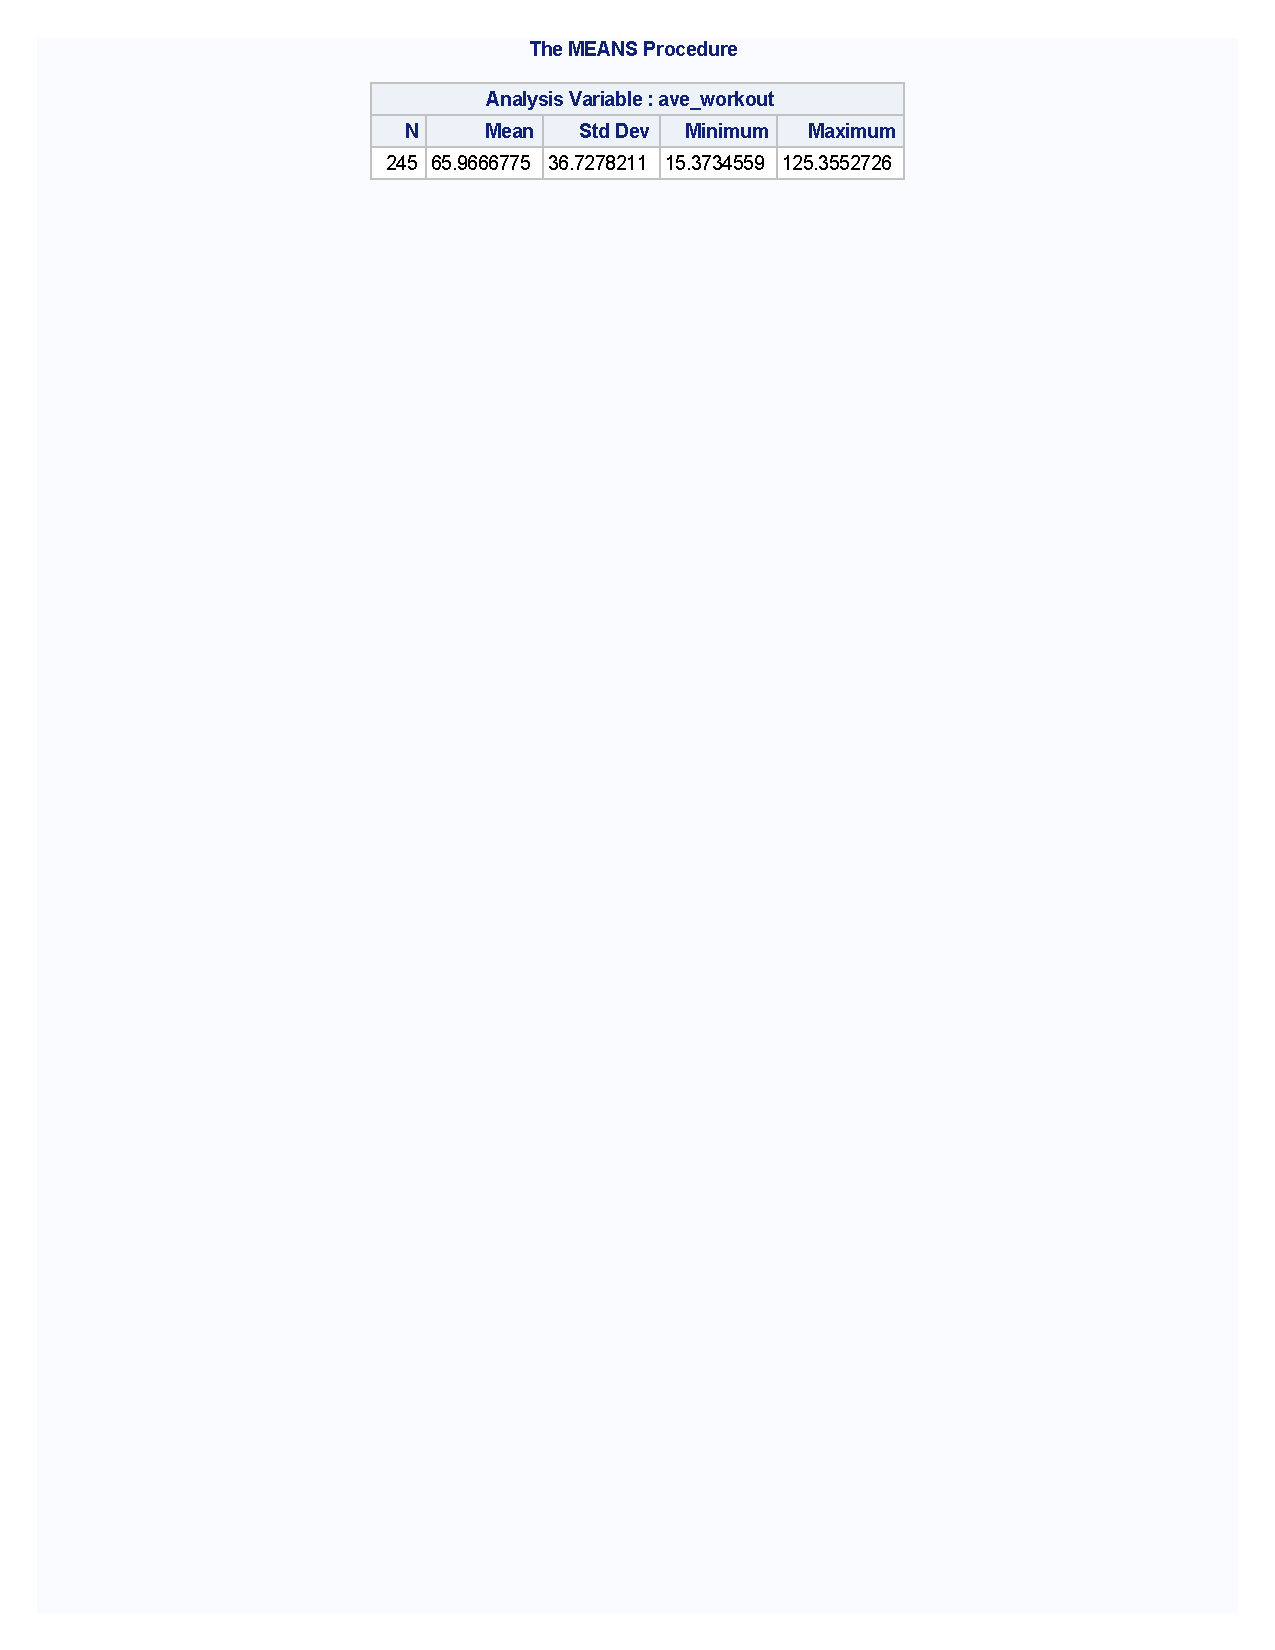
\includegraphics[trim={4cm 23cm 4cm 0.5cm},clip]{q7.pdf}
\item \emph{In your data step:} There are a series of question 3 items that corresponded to a single ``Mark all that apply'' type question.  Utilize these responses to create a new variable called \texttt{prev\_stats} which has a value of \texttt{yes} if students have previous experience with statistics and a value of \texttt{no} if the student does not have previous experience with statistics.  \emph{Hint: it may be helpful to discuss a `game plan' with neighboring students or the instructor prior to coding.}
\item \emph{Under the data step, using your permanent SAS data set:} Apply PROC FREQ to the \texttt{prev\_stats} variable to determine how many students had previous experience with statistics.  Your output should match the output shown below.
\item[]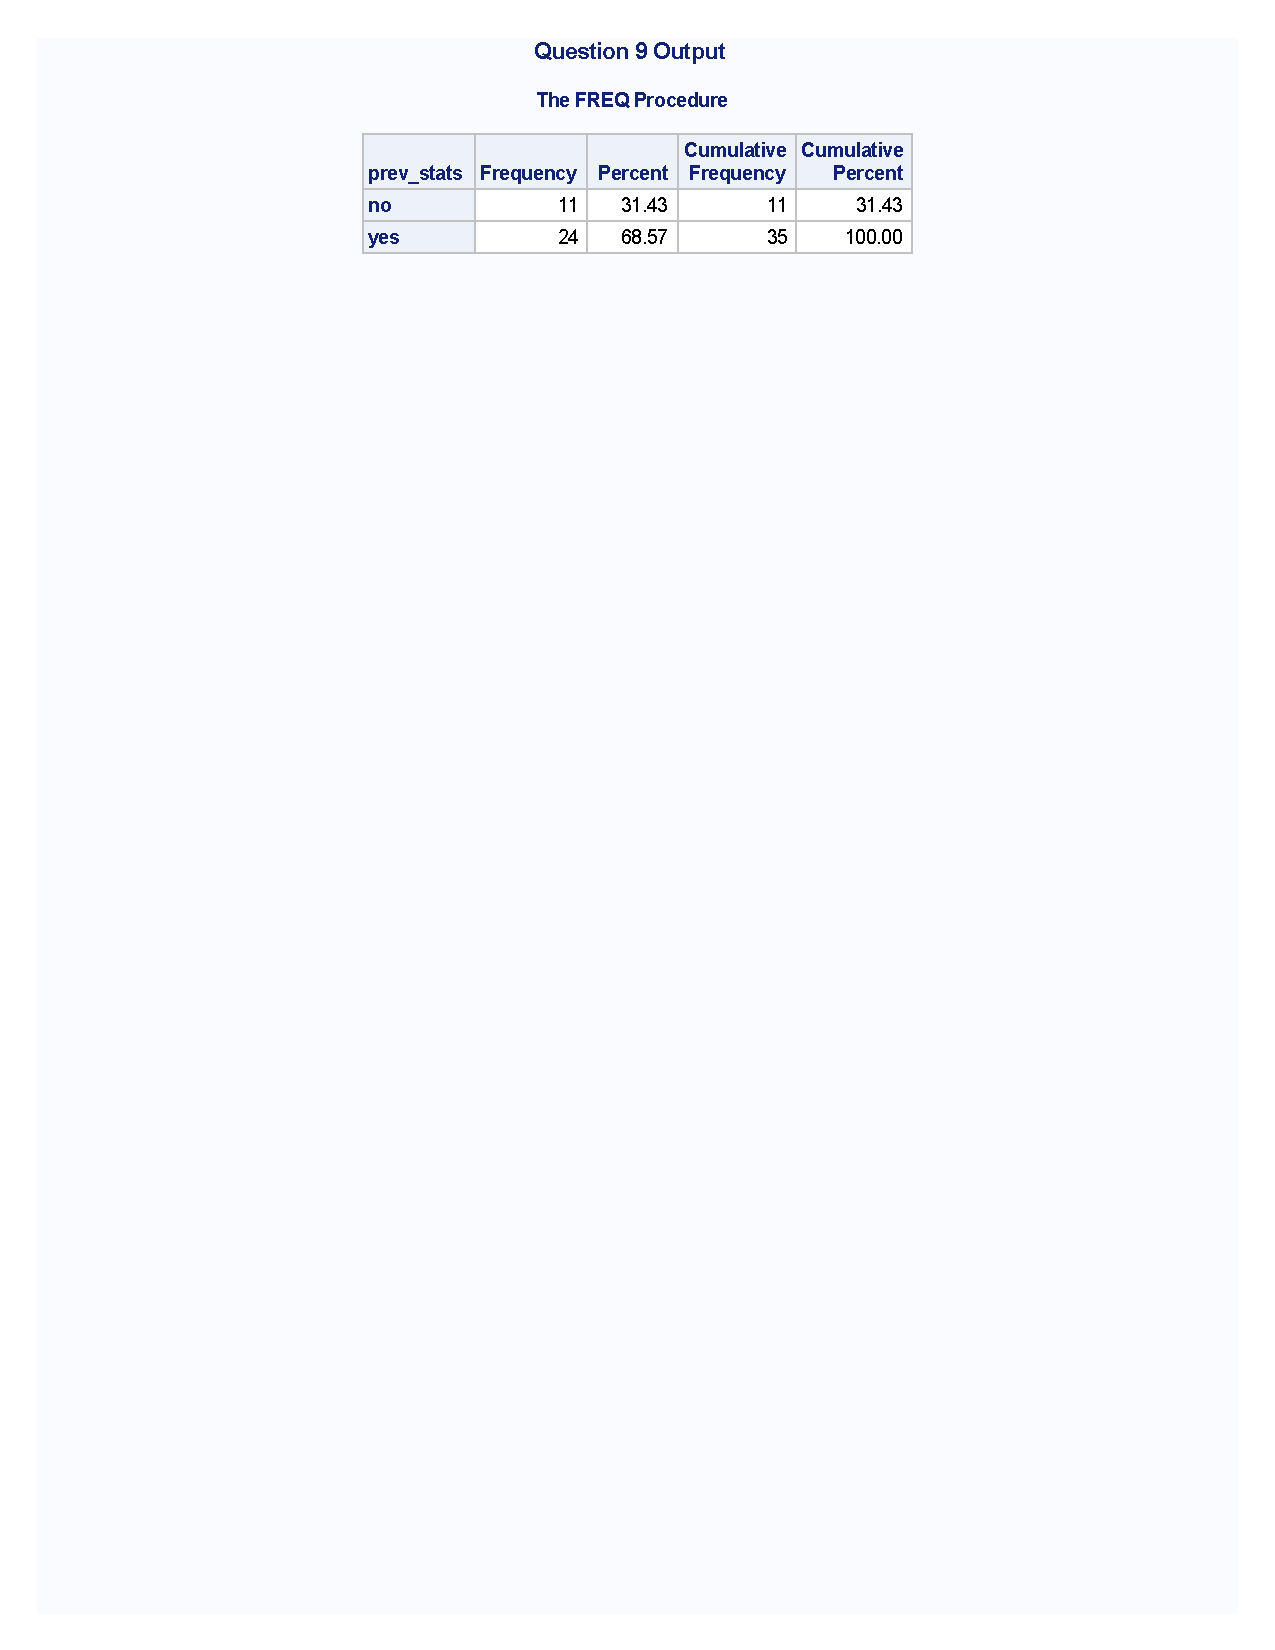
\includegraphics[trim={4cm 23cm 4cm 0.5cm},clip]{q9.pdf}
\item  \emph{Under the data step, using your permanent SAS data set:}  Utilize a procedure that summarizes all of the values regarding year at Cal Poly.
\item \emph{In your data step:}  Create a new variable called \texttt{class} that classifies students as ``lower'' class (first years and second years) and ``upper'' class (third years, fourth years, etc.).
\item  \emph{Under the data step, using your permanent SAS data set:}  Apply PROC FREQ to the \texttt{class} variable to determine how many lower and upper class students are enrolled.  Your output should match the output shown below.
    \item[]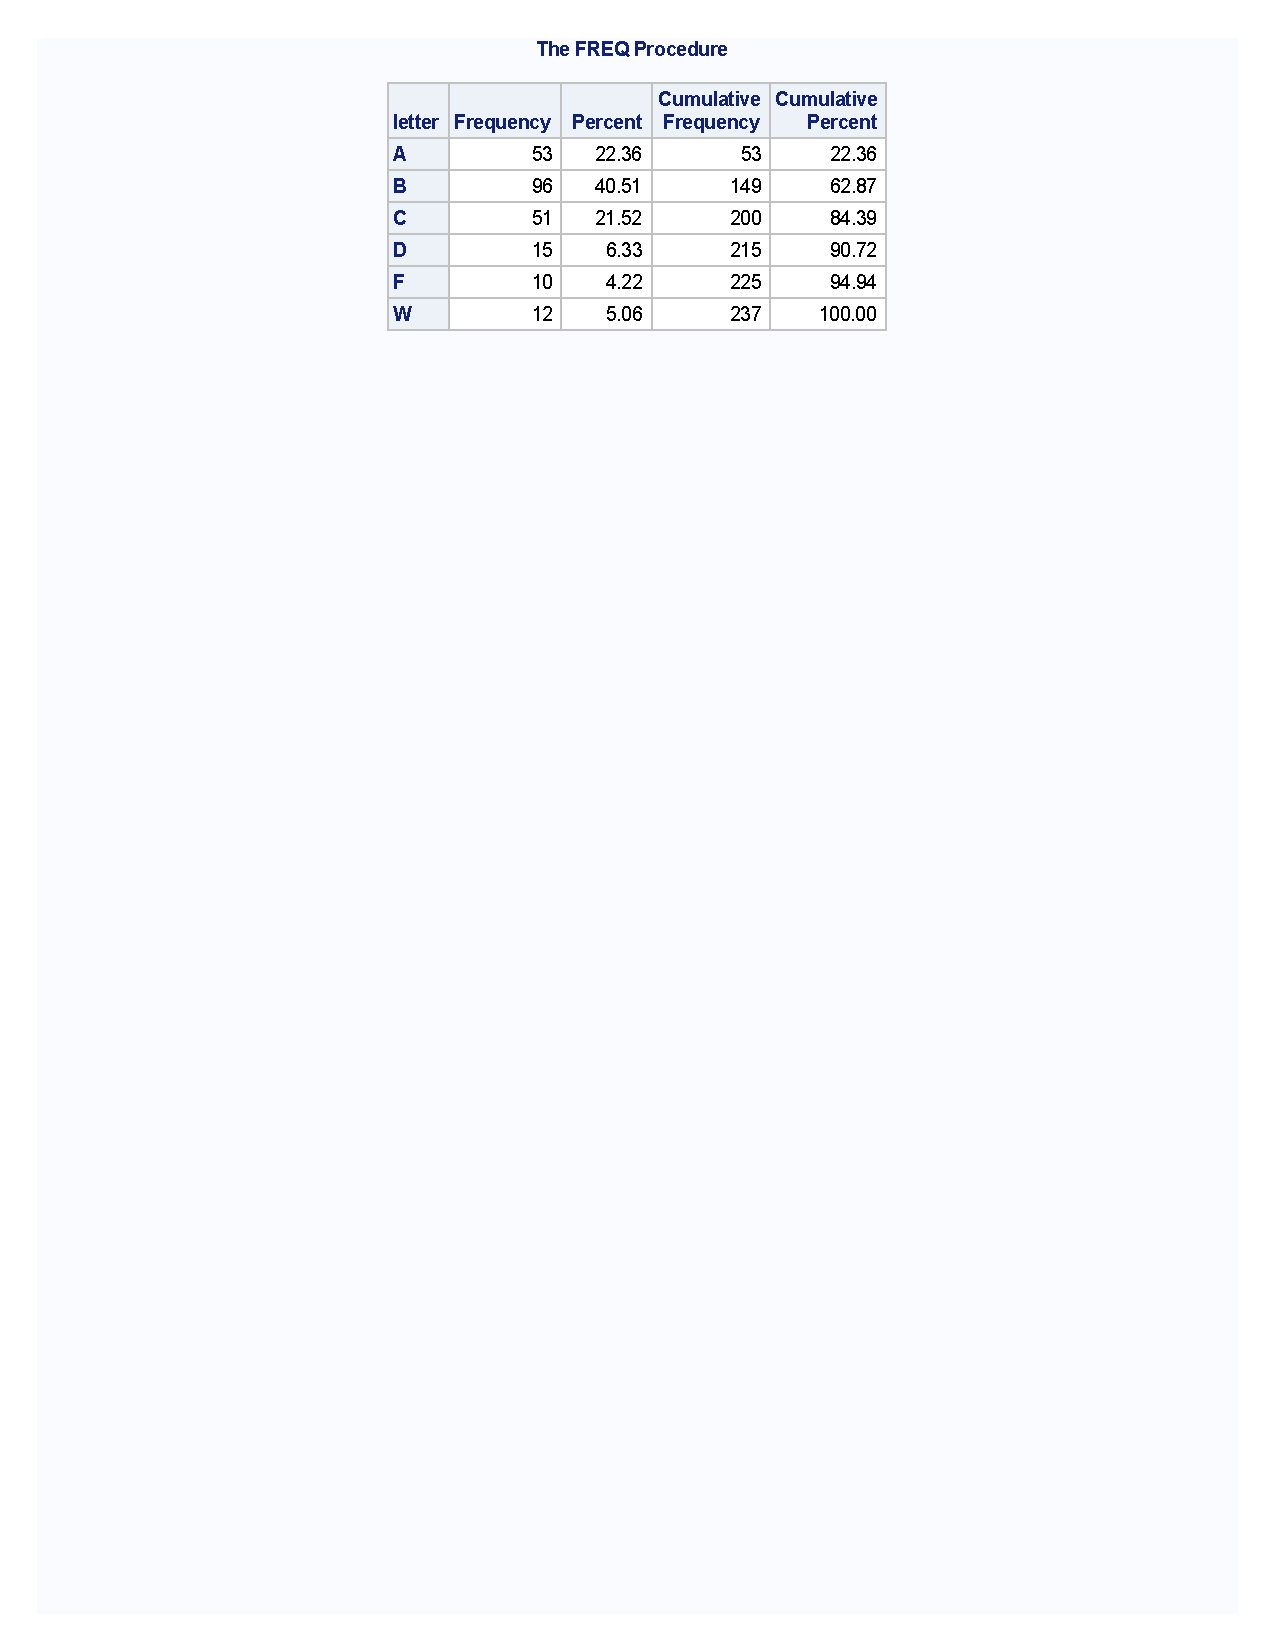
\includegraphics[trim={4cm 23cm 4cm 0.5cm},clip]{q11.pdf}
\item \emph{In your data step:}  According to the registrar's office, graduation with honors are awarded as follows:
\begin{itemize}
\item \emph{Summa cum laude:} cumulative Cal Poly GPA of 3.85 or higher
\item \emph{Magna cum laude:} cumulative Cal Poly GPA of 3.70 to 3.84
\item \emph{Cum laude:} cumulative Cal Poly GPA of 3.50 to 3.69
\end{itemize}
Use the \texttt{GPA\_clean} variable to create a new variable called \texttt{honors} that classifies students according to their current GPA; students who do not yet achieve honors should be classified as ``none''.  Students with a missing value for \texttt{GPA\_clean} should also have a missing value for \texttt{honors}.
\item \emph{Under the data step, using your permanent SAS data set:}  Apply PROC FREQ to the \texttt{honors} variable to determine the distribution of honors.  Your output should match the output shown below.
\item[]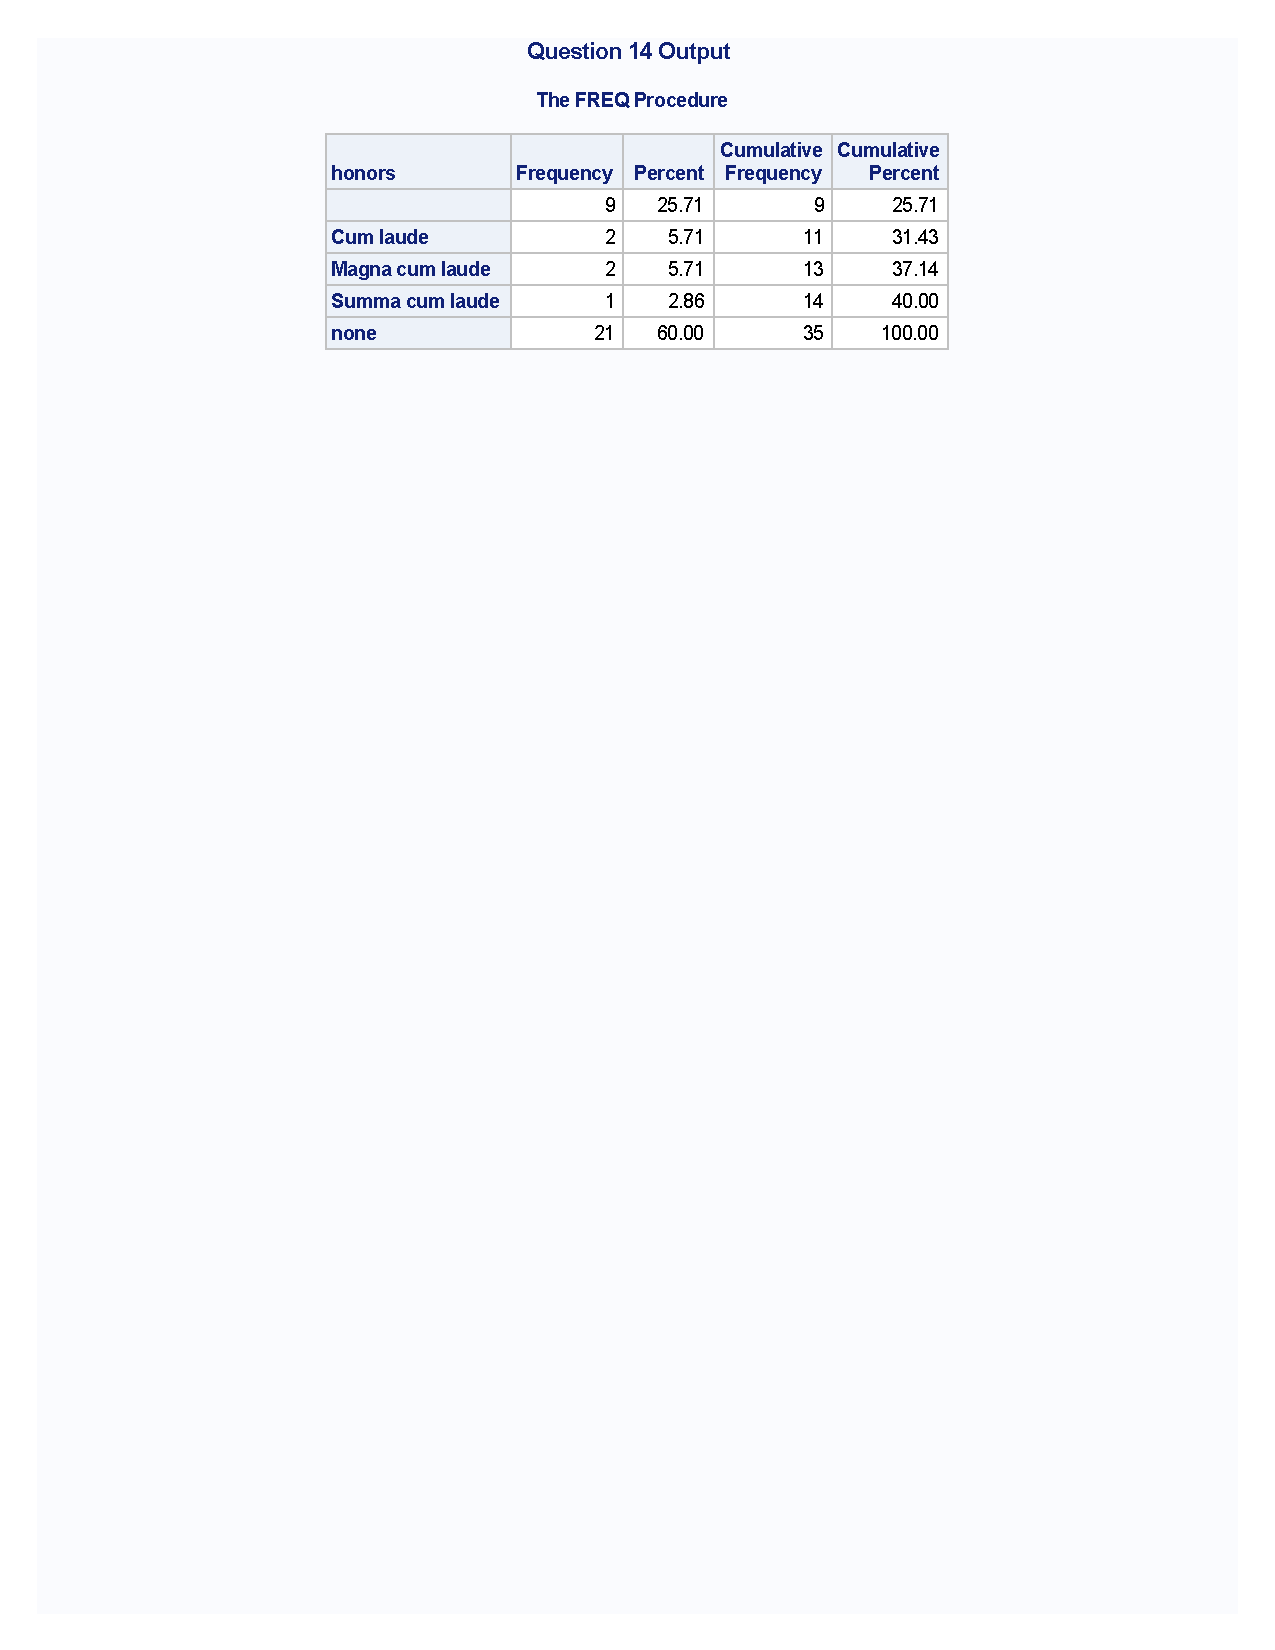
\includegraphics[trim={4cm 21cm 4cm 0.5cm},clip]{q14.pdf}
\item When I ask students to tell me something about themselves, many say that they enjoy the outdoors.  Identify a SAS function that can look for phrases in a character string.  Use this function to create a new variable called \texttt{outdoors} which should have a value of ``yes'' if their statement includes the word ``outdoors'' and a value of ``no'' otherwise.
\item \emph{Under the data step, using your permanent SAS data set:}  Apply PROC FREQ to the \texttt{outdoors} variable to determine how many students mentioned the outdoors in their statement.  Your output should match the output shown below.
\item[]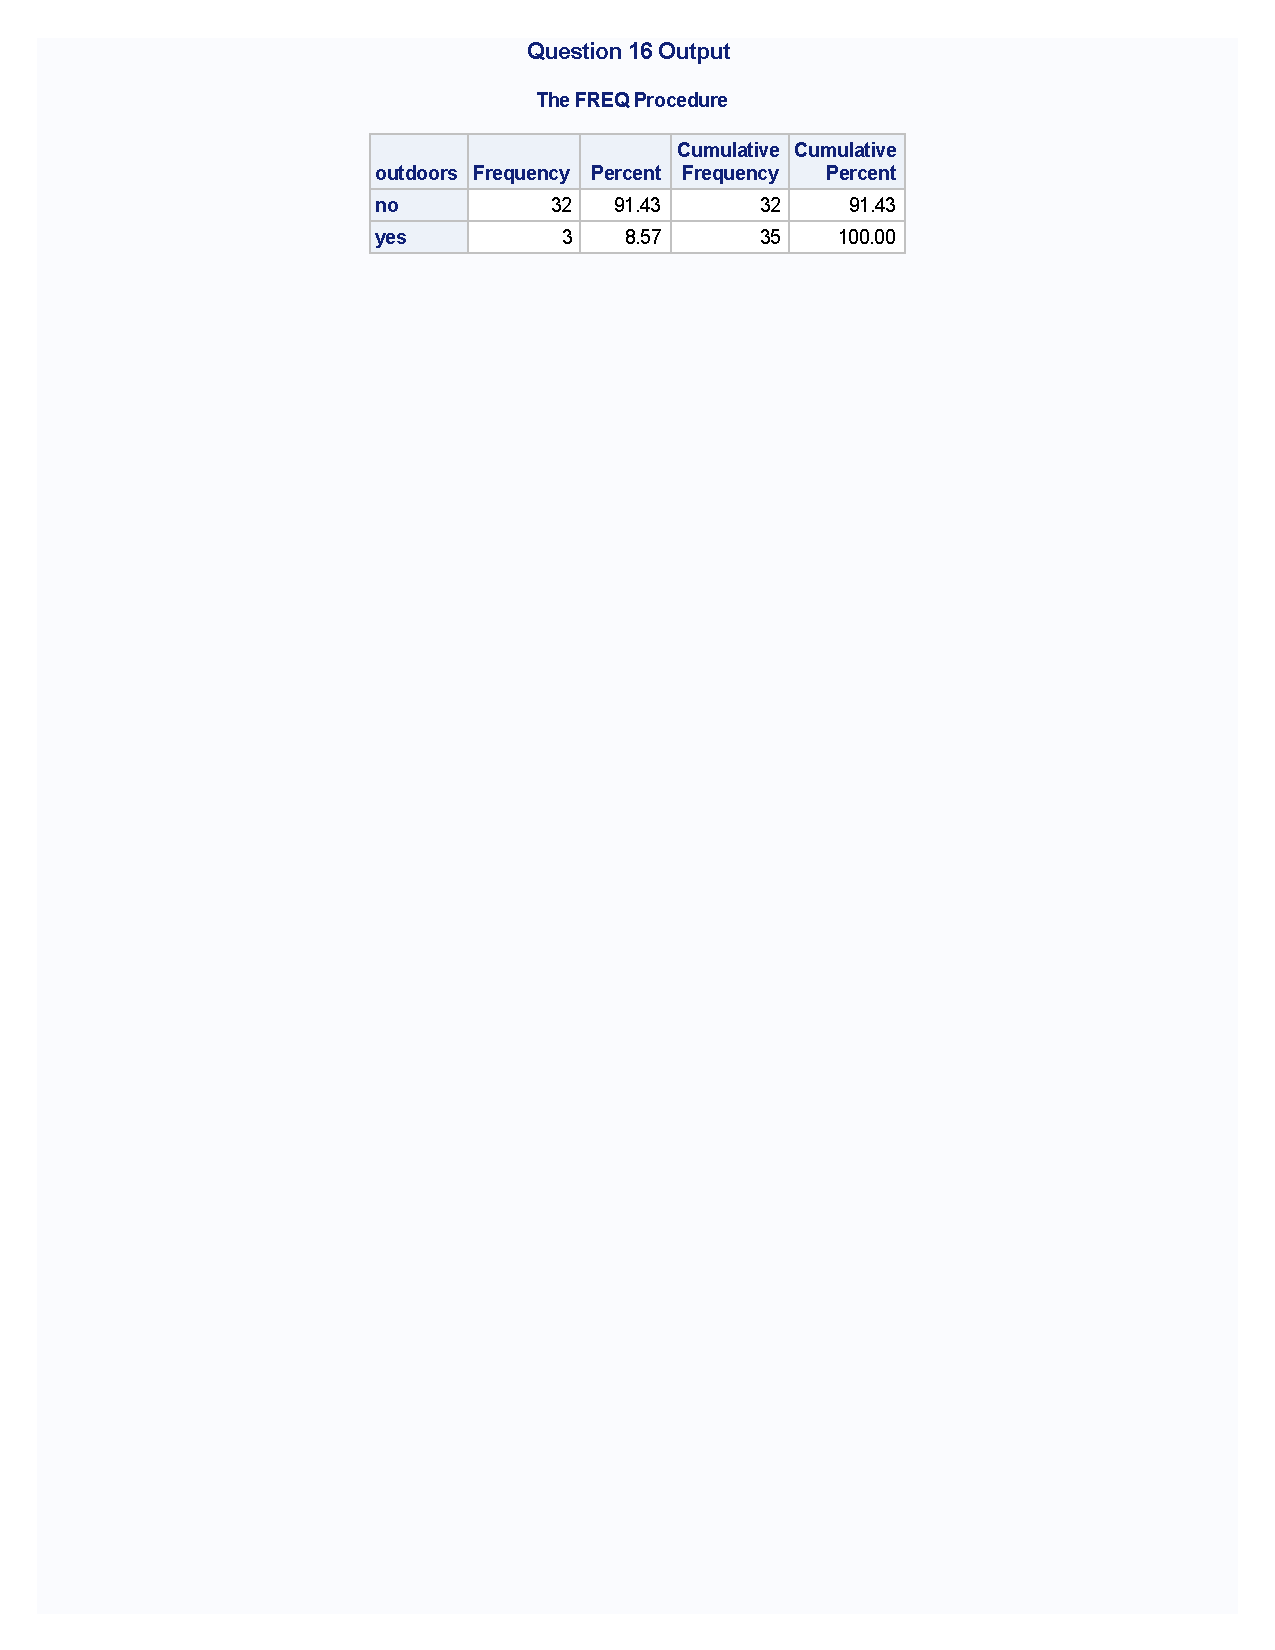
\includegraphics[trim={4cm 22cm 4cm 0.5cm},clip]{q16.pdf}
\item \emph{After your last PROC:} Create a new, temporary SAS data set called \texttt{shortlist} that contains only the five students with honors and only two variables: honors and how they take notes.  Apply a PROC PRINT to this data set to view it.  Your output should match the output shown below.
\item[]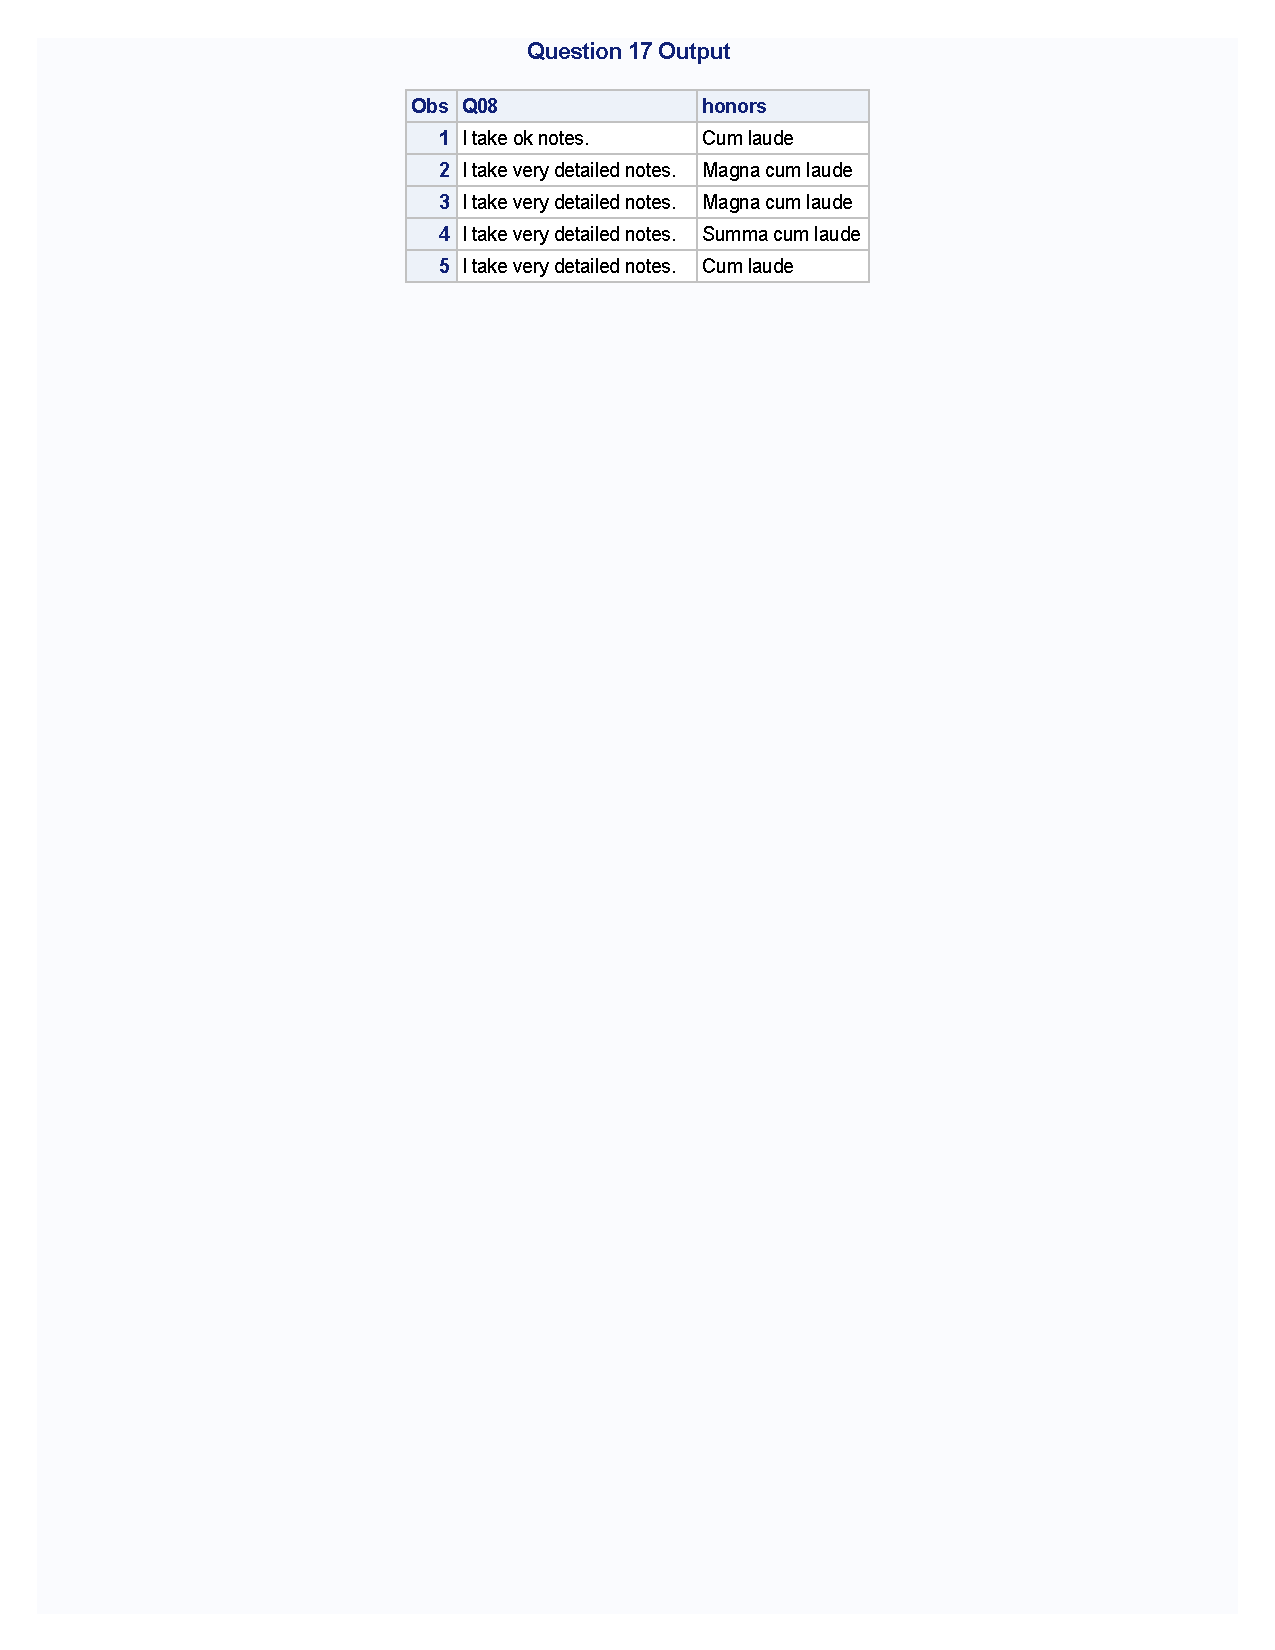
\includegraphics[trim={4cm 22cm 4cm 0.5cm},clip]{q17.pdf}
\end{enumerate}

\end{document} 